%
% Copyright (c) 2017  Zubax Robotics OU  <info@zubax.com>
%
% Distributed under BY-NC-ND (attribution required, non-commercial use only, no derivatives).
%

\documentclass{zubaxdoc}
\usepackage{svg}
\graphicspath{{document_templates/documentation_template_latex/}}

\title{Zubax Babel Datasheet}

\begin{document}
\frontmatter
\begin{titlepage}
\section*{Overview}
Zubax Babel is an advanced USB-CAN and UART-CAN adapter that can be used as a standalone device or as an embeddable module for OEM. It features a software-controlled termination resistor, embedded bus power supply and bus voltage monitoring. Zubax Babel uses the quasi-standard SLCAN (aka LAWICEL) protocol (with Zubax extensions) for transferring CAN data over serial port.

\section*{Features}

The adapter has a number of important features that are rarely seen in competing designs:
\begin{itemize}
\item Low latency - cumulative latency between the USB CDC ACM interface on the host system and the CAN bus is under 1 millisecond. Tested with USB connection on desktop Linux 3.13 using low-latency SLCAN driver from PyUAVCAN.
\item High throughput - the device handles over 5000 frames per second in either direction continuously. Tested with USB connection on desktop Linux 3.13. When using UART interface, the throughput of the device is limited by the UART baud rate.
\item Proper prioritization of outgoing CAN frames. The adapter properly schedules the outgoing frames, avoiding the inner priority inversion in the TX queue.
\item Large RX buffer (255 CAN frames plus 2KB of serial buffers) allows the device to handle short-term traffic bursts without frame losses when interfaced via low-speed UART.
\end{itemize}

\BeginRightColumn

\section*{Applications}

Zubax Babel is primarily intended for UAVCAN applications, although other CAN bus protocols are supported equally well. We recommend the UAVCAN GUI Tool for use with Zubax Babel; however, there is a wide selection of software products that can talk with SLCAN adapters and therefore are compatible with Zubax Babel too.

\centering
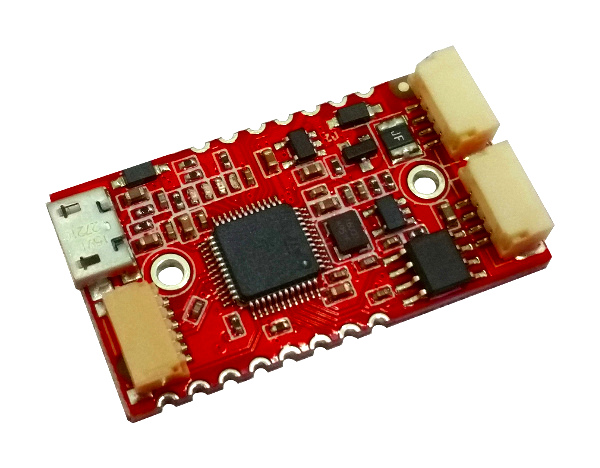
\includegraphics[width=0.45\textwidth]{top}
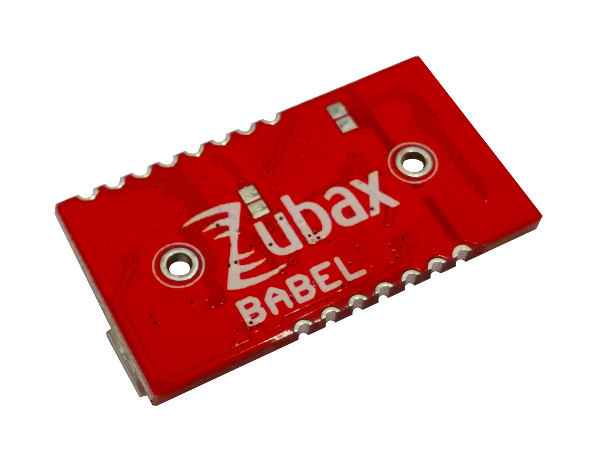
\includegraphics[width=0.45\textwidth]{bottom}

\end{titlepage}

\tableofcontents
\BeginRightColumn
\listoffigures
\listoftables


\mainmatter

\chapter{Overview}

Zubax Babel is an advanced USB-CAN and UART-CAN adapter that can be used as a standalone device or as an embeddable module for OEM. It features a software-controlled termination resistor, embedded bus power supply and bus voltage monitoring. Zubax Babel uses the quasi-standard SLCAN (aka LAWICEL) protocol (with Zubax extensions) for transferring CAN data over serial port.

\section{System integration}

Zubax BABEL is powered from USB or oprional SMD pads. It can provide power(up to 500mA) to UAVCAN bus via software controlled key.  
The 5 V rail of the CAN interface us not used by the device; 5 V rails of CAN connector pair are connected directly together.

\section{Enclosure}\label{sec:enclosure}

Zubax Babel is intended for integration into the end system in the form of the bare PCB,
as this facilitates lower weight and tighter arrangement of components
in the end device, all of which are desirable properties in the target application domains.

Shall it be desired to provide additional mechanical protection for the device or to use it as generic diagnostic adapter, the plastic enclosure pictured on the figure \ref{enclosure} can be used.
Please contact your supplier for the ordering information;
alternatively, visit \url{https://github.com/Zubax/zubax_babel/} to download
3D printable enclosure models suitable for in-house manufacturing.

\begin{figure}[hb]
	\centering
	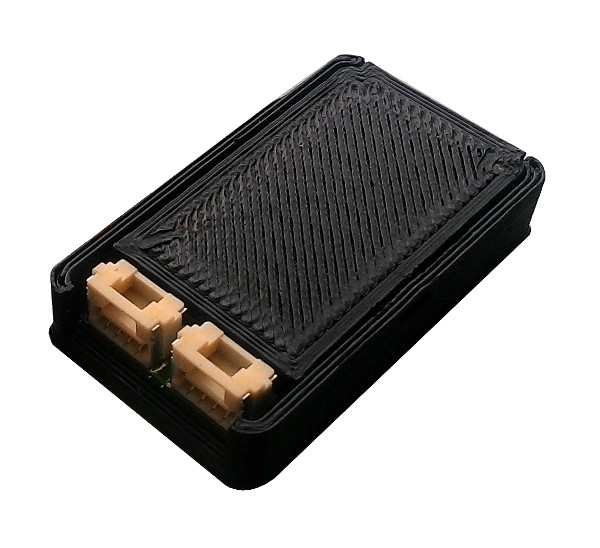
\includegraphics[width=0.45\textwidth]{housing}
	\caption{Plastic enclosure.\label{enclosure}}
\end{figure}

\chapter{Characteristics}

\section{General electrical characteristics}

\begin{ZubaxSimpleTable}{Environmental conditions}{|c |l c|c|X|}
     Parameter &  Min & Max & Unit  & Note \\
	 Board temperature & -40 & 70 & \degree{}C & \\
	 Relative humidity & 0 & 100 &\%RH & Non-considering 
\end{ZubaxSimpleTable}

\begin{ZubaxSimpleTable}{Power}{|c | c | c | c | c | X | }
Parameter & Minimum & Typical & Maximum & Units & Note \\
Supply voltage & 4.0 & 5.0 & 5.5 & V & Any power input \\ 
Supply current & 30 & 50 & 80 & mA & SMD pads floating, UART and SWD lines floating \\
3.3 V rail output voltage & 3.2 & 3.3 & 3.4 & V & \\
3.3 V rail external load &  & & 100 & mA & \\
\end{ZubaxSimpleTable}

\begin{ZubaxSimpleTable}{CAN bus}{| X | c | c | c | c | }
Parameter & Minimum & Typical & Maximum & Units \\
Supported baud rates &	2400 & 115200 & 	3000000	& baud/s \\
Low-level input voltage &	-0.3 &	0 &	1.6 &	V \\
High-level input voltage &	2.1 &	3.3 & 5.5 & 	V \\
Low-level output voltage &	0 &	0 &	0.5 &	V \\
High-level output voltage & 2.8 & 3.3 & 3.4 &	 V \\
Source/sink current (magnitude)  & & &			10 &	mA \\
\end{ZubaxSimpleTable}

\begin{ZubaxSimpleTable}{SMD signal pads}{| X | c | c | c | c | }
Parameter & Minimum & Typical & Maximum & Units \\
Low-level input voltage & -0.3 & 0 & 1.6 & V \\
High-level input voltage & 2.1 & 3.3 & 5.5 & V \\
Low-level output voltage & 0 & 0 & 0.5 & V \\
High-level output voltage & 2.8 & 3.3	& 3.4	& V \\
Source/sink current (magnitude) & & 10 & & mA \\
\end{ZubaxSimpleTable}
\clearpage
\section{Mechanical characteristics}
The drawing below documents the basic mechanical characteristics of Zubax Babel, such as the placement of connectors and mounting holes:

\begin{figure}[!hbt]
	\centerline{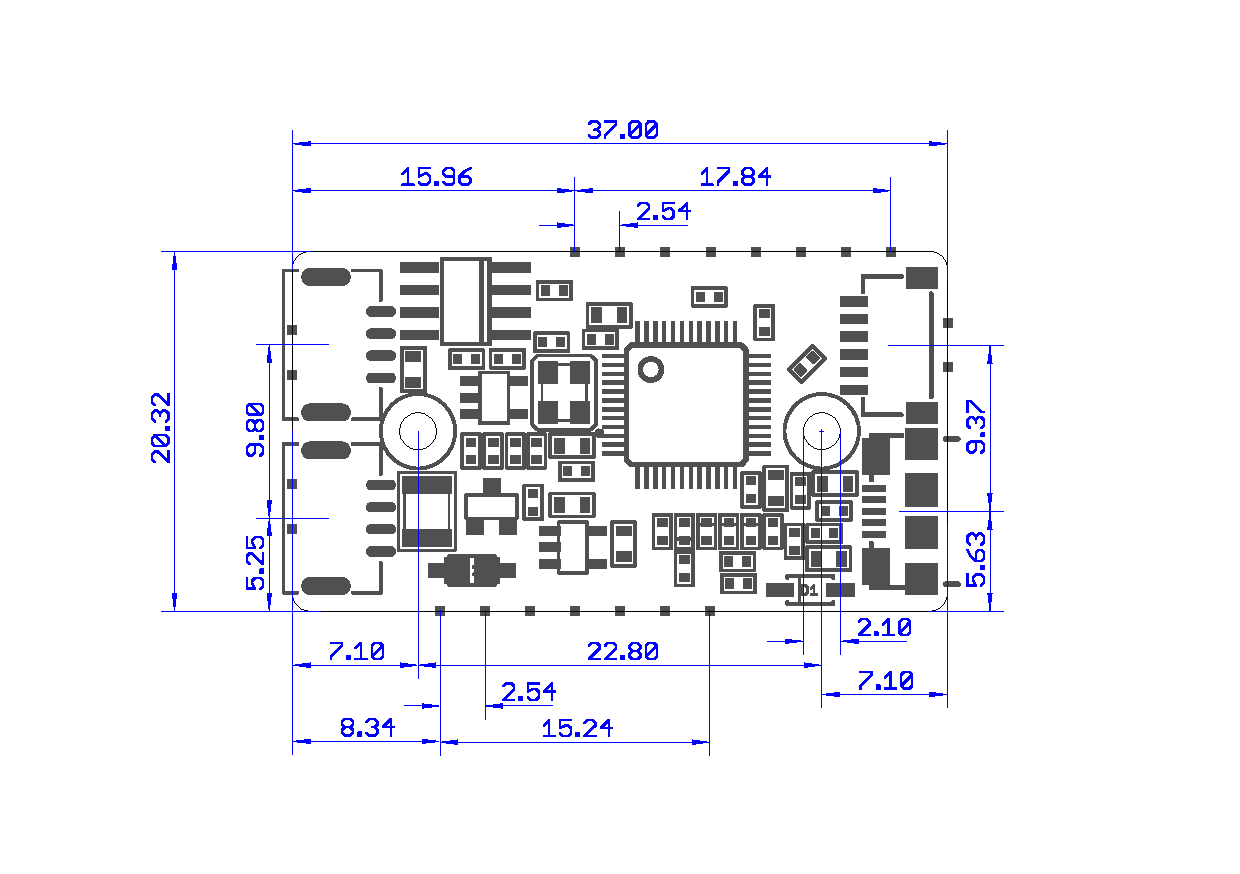
\includegraphics[width=1.1\textwidth]{babel_dimensions}}
	\caption{Babel drawing.\label{drawing}}
\end{figure}

\clearpage
Pinout is shown on the diagram:
\begin{figure}[!hbt]
	\centerline{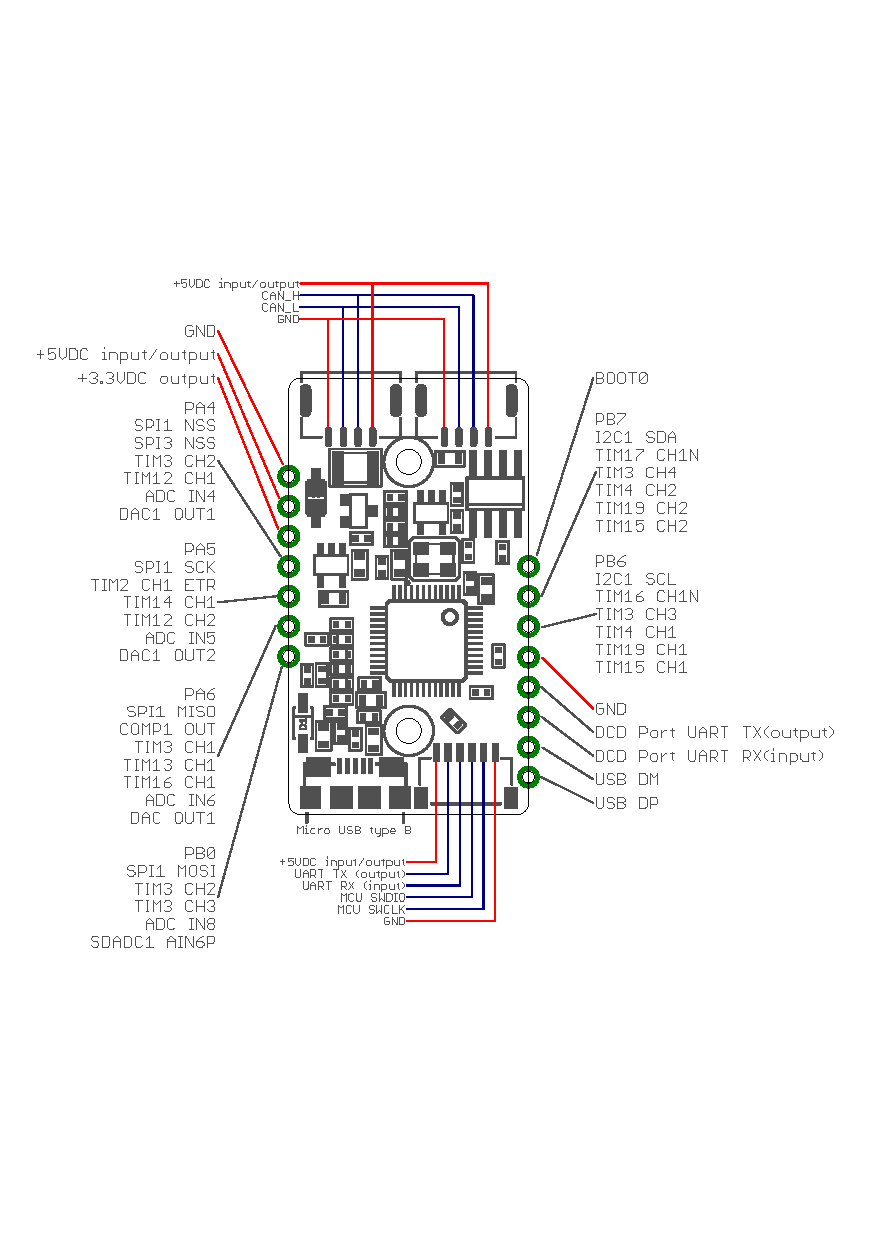
\includegraphics[width=1\textwidth]{babel_pinout}}
	\caption{Babel pinout.\label{pinout}}
\end{figure}

\chapter{Power supply}

The device is powered by +5 VDC which can be delivered via any (or multiple) of the interface connectors:
\begin{itemize}
\item USB connector (input only)
\item CAN connectors (input, optional output)
\item DroneCode Debug Port connector (input and output)
\item SMD pads (input and output)
\end{itemize}

The device has a reverse current protection on the USB power input, to prevent back-powering the USB host when it is turned off. The CAN power output has a solid state switch that can be enabled and disabled programmatically (more on this in the later sections); however, the device can be powered from the CAN bus regardless of the state of the power switch. Additional 3.3VDC output on the SMD pads can be used to power the external circuit when the device is used in OEM mode. See the following diagram:
\\ \\
\begin{figure}[!hbt]
	\centerline{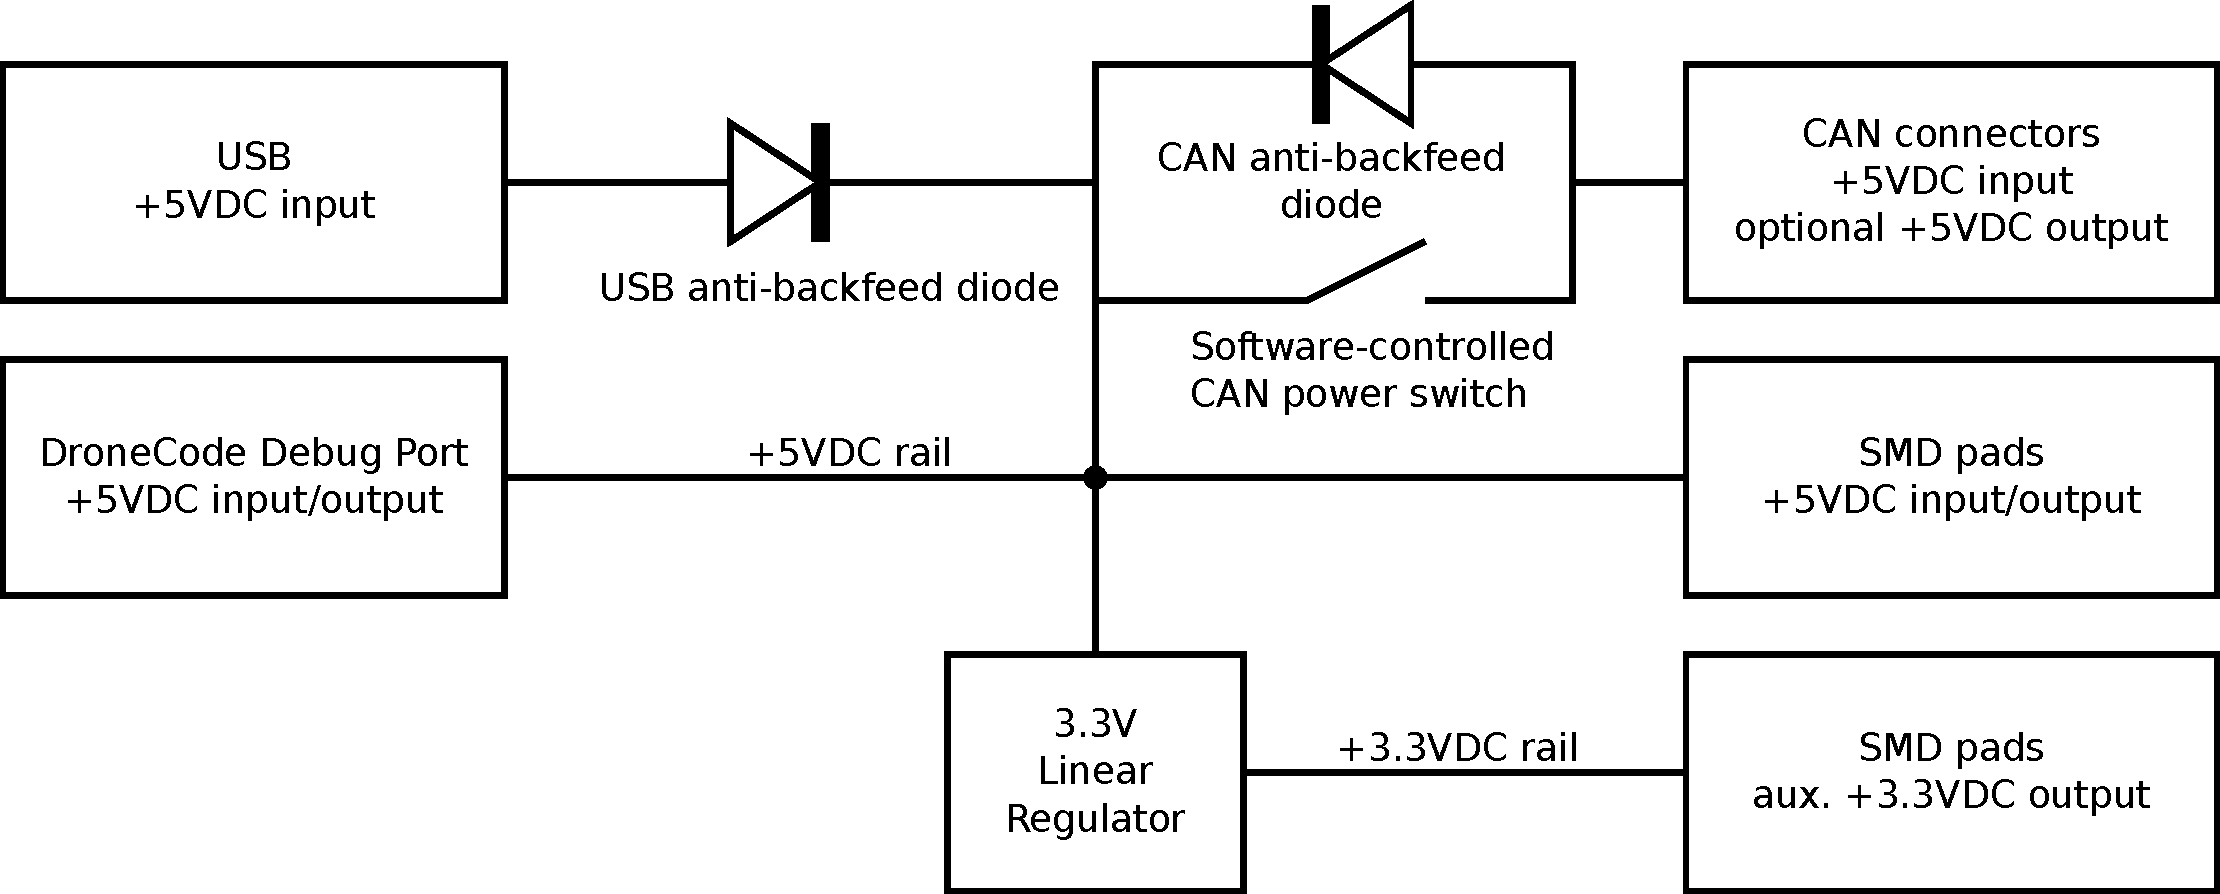
\includegraphics[width=1\textwidth]{power_supply}}
	\caption{power supply scheme.\label{power supply scheme}}
\end{figure}

\chapter{LED indicators}

\begin{ZubaxSimpleTable}{Led indicators}{| l |  X |}
Color & Indicates \\
Red & CAN power switch is turned ON \\
Orange & 120$\Omega$ CAN terminator ON \\
Blue & Status, see below \\
Green & Blinks once if there was at least one CAN frame successfully sent or received in the last 25 milliseconds. This feature allows the user to visually evaluate the load of the CAN bus.
\end{ZubaxSimpleTable}

The status LED (blue) behaves as follows:

\begin{ZubaxSimpleTable}{Status LED behavior}{| l |  X |}
Status & Pattern \\
Bootloader is running & Glowing continuously \\
CAN channel is closed & Turned OFF \\
CAN channel is open and operating normally & Blinking 1 Hz (slowly) \\
CAN channel is open, CAN error passive & Blinking 4 Hz (quickly) \\
CAN channel is open, CAN bus off & Blinking 10 Hz (very quickly) \\
\end{ZubaxSimpleTable}

While the bootloader is running, the traffic LED (green) is used to indicate the bootloader\textquotesingle s status as follows:

\begin{ZubaxSimpleTable}{Bootloader status indication}{| l |  X |}
Status & Pattern \\
Ready to boot, or waiting for boot delay expiration & Turned OFF\\
Boot cancelled by external request (e.g. CLI command) & Blinking 1 Hz, short pulses (50 ms) \\
Application upgrade is in progress & Blinking 1 Hz, long pulses (500 ms) \\
No valid application found, boot is not possible & Blinking 10 Hz (very quickly) \\
\end{ZubaxSimpleTable}

\chapter{Interfaces}
\section{USB}

Zubax Babel exposes a USB CDC ACM interface (a.k.a. virtual serial port) via full-speed USB 2.0 port. For more information about the serial port and appropriate drivers, please refer to the dedicated article.

The device implements the SLCAN protocol with custom extensions on top of the CDC ACM interface, which is documented in the later sections.

Note that while USB is connected, the UART interface of the DroneCode Debug Port is not available. In order to use UART, USB must be disconnected.

\section{DroneCode Debug Port}

The DroneCode Debug Port exposes the standard ARM SWD interface and a UART port. The UART port exposes a CLI. Same SLCAN protocol operates on top of the UART CLI as on the USB CLI.

Note that while USB is connected, the UART interface of the DroneCode Debug Port is not available. In order to use UART, USB must be disconnected.

\section{CAN bus}
Zubax Babel implements ISO 11898, also known as high-speed CAN. The CAN interface recovers from bus-off and other error states automatically.

The CAN bus interface is exposed via two parallel 4-pin JST GH connectors. These are the standard UAVCAN Micro Connectors.

The device has an embedded 120$\Omega$ termination resistor that can be enabled and disabled via the SLCAN interface.

The power switch, when turned on, delivers the +5 VDC supply to the CAN bus, which can be used to power other CAN bus nodes from Zubax Babel (see the power system diagram).

\section{SMD pads}

Please refer to the OEM section below.

\chapter{SLCAN protocol}

SLCAN (also known as LAWICEL) is a quasi-standard protocol designed for tunneling CAN data (frames, commands and adapter status information) via serial links (UART or USB CDC ACM). Zubax Babel implements all mandatory SLCAN commands, so that its compatibility with third party software products that rely on SLCAN is ensured. A brief recap of standard SLCAN commands, prepared by Oliver Hartkopp, can be found in this document: \href{https://docs.zubax.com/zubax_babel/Generic_SLCAN_API.pdf}{Generic\_SLCAN\_API.pdf}.

SLCAN is an ASCII protocol, where the data is exchanged in blocks, each block may contain only printable ASCII characters and is terminated with either ACK (\fbox{$\backslash$r}, ASCII code 13) or NACK (\fbox{$\backslash$a}, ASCII code 7). Every block begins with a well-defined character which indicates what information the block is carrying; in this description we’re going to refer to this character as Block ID. Three types of blocks are defined:

\begin{itemize}
\item Command - these blocks are sent from the host to the adapter.
\item Response - these blocks are sent from the adapter to the host as a reaction to the corresponding command. Any command always results in exactly one response.
\item Indication - these blocks are generated by the adapter itself asynchronously.
\end{itemize}

All commands and indications are always terminated with ACK (\fbox{$\backslash$r}). A response will be terminated with ACK if the command was executed successfully, and with NACK if the command failed or if the command ID could not be mapped to any known command handler.

Zubax Babel also implements an extension on top of SLCAN that allows the host to execute arbitrary CLI commands, sharing the same serial port with SLCAN. This feature is documented later in this section.

Note that some commands alter the configuration parameters of the adapter. All parameters can be stored into the non-volatile memory on the adapter, in which case they will be re-initialized to the saved values autimatically every time the adapter is turned on. The non-volatile memory feature is explained later in this section.

Keep in mind that Zubax Babel can be communicated with either via USB or via the DCD Port (UART), but not both at the same time. When USB is connected, only USB is used, the UART port is ignored. In order to use UART, USB must be disconnected.

Decent implementation of a host-side SLCAN driver in Python can be found in the \href{http://uavcan.org/Implementations/Pyuavcan/}{PyUAVCAN library}.
\clearpage
\section{SLCAN commands}
\subsection{CAN controller configuration}

\begin{ZubaxSimpleTable}{CAN controller configuration}{| l |  l | X |}
Block ID & Arguments & Purpose \\
\fbox{S} & 	Decimal number, see below & Set CAN bitrate. \\
\fbox{O} & None & Open CAN channel at the specified earlier bitrate in normal mode; re-open if already open. \\
\fbox{L} & None & Open CAN channel at the specified earlier bitrate in silent mode (listen only); re-open if already open. \\
\fbox{l} & None & Open CAN channel at the specified earlier bitrate in normal mode with loopback enabled; re-open if already open. \\
\fbox{C} & None & Close CAN channel; do nothing if channel is not open. \\
\fbox{M} & Any, not checked & This command is not applicable for Zubax Babel, it is implemented only for compatibility reasons. \\
\fbox{m} & Any, not checked & See \fbox{M}
\end{ZubaxSimpleTable}

All commands return \fbox{$\backslash$r} on success and \fbox{$\backslash$a} on failure. Commands that are implemented for compatibility always report success.

The command \fbox{S} accepts a non-negative decimal number which represents the desired CAN bitrate. If the channel is open, changes in bitrate will not take effect until it’s re-open again. The values are interpreted as follows:

\begin{ZubaxSimpleTable}{CAN bitrate}{| l |  X |}
Value & Interpretation, bits per second \\ 
0 & 10000 \\
1 & 20000 \\
2 & 50000 \\
3 & 100000 \\
4 & 125000 \\
5 & 250000 \\
6 & 500000 \\
7 & 800000 \\
8 & 1000000 \\
Any other & The number is interpreted as-is, no additional conversion is performed.\\
\end{ZubaxSimpleTable}

When the channel is open with loopback enabled, all transmitted frames will be sent back to the host, with the loopback flag set (if SLCAN flags are enabled). See more on this in the section dedicated to SLCAN indications.

\subsection{CAN frame transmission}

In the command table, arguments are indicated as defined in the table below. Valid hexadecimal characters are the following:  \fbox{0123456789} \fbox{abcdef} \fbox{ABCDEF}.

\begin{ZubaxSimpleTable}{SLCAN arguments meaning}{| l |  X |}
Symbol & Meaning\\
\fbox{i} & 	Hexadecimal digit of a CAN ID \\
\fbox{d} & Hexadecimal DLC(Data Length Code) value \\ 
\fbox{*} & Useful data, encoded as a hexadecimal string, e.g. \fbox{0110FF} for the following sequence: 1, 16, 255. \\
\end{ZubaxSimpleTable}

\begin{ZubaxSimpleTable}{SLCAN command format}{| l |  l | l | X |}
Block ID & Arguments & Purpose & Example \\
\fbox{T} & \fbox{iiiiiiiid*} & Transmit 29-bit data frame & \fbox{T0123456780102030405060708$\backslash$r}\\
\fbox{t} & \fbox{iiid*} & Transmit 11-bit data frame & \fbox{t7FF0$\backslash$r}\\
\fbox{R} & \fbox{iiiiiiiid} & Transmit 29-bit RTR frame & \fbox{R1234f00d8$\backslash$r}(RTR frames have no payload)\\
\fbox{r} & \fbox{iiid} & Transmit 11-bit RTR frame & \fbox{r008$\backslash$r}(RTR frames have no payload)\\
\end{ZubaxSimpleTable}

All above listed commands may generate the following responses:

\begin{ZubaxSimpleTable}{Possible responses}{| l |  X |}
Response & Meaning \\
\fbox{Z$\backslash$r} & The frame has been successfully scheduled for transmission (for 29-bit ID) \\
\fbox{z$\backslash$r} & The frame has been successfully scheduled for transmission (for 11-bit ID) \\
\fbox{$\backslash$a} & The adapter could not transmit the frame (e.g. malformed frame, CAN channel is not open, etc.)\\
\end{ZubaxSimpleTable}

\subsection{Miscellaneous commands}
\begin{ZubaxSimpleTable}{Miscellaneous commands}{| l |  l | X |}
Block ID & Arguments & Purpose \\
\fbox{U} & Decimal number, see below & Set UART baud rate \\ 
\fbox{Z} & \fbox{0} or \fbox{1} & Enable (if 1) or disable (if 0) RX and loopback timestamping \\
\fbox{F} & None & Get and clear status flags \\ 
\fbox{V} & None & Get hardware and software version \\
\fbox{N} & None & Get unique ID (conventional SLCAN adapters return the serial number, which Zubax products may not have) \\
\end{ZubaxSimpleTable}

\clearpage

The command \fbox{U} accepts a non-negative decimal number which represents the desired UART baud rate. Changes will take effect shortly after the command was executed (typically within 100 milliseconds), no reboot is necessary; therefore, the host should adjust the baud rate of the serial port immediately after execution of this command. The number is interpreted as follows:

\begin{ZubaxSimpleTable}{Baudrate codes}{| l |  X |}
Value & Interpretation, baud per second \\
0 & 230400 \\ 
1 & 115200 \\
2 & 57600 \\
3 & 38400 \\
4 & 19200 \\
5 & 9600 \\
6 & 2400 \\
Any other & The number is interpreted as-is, no additional conversion is performed.
\end{ZubaxSimpleTable}

The following baud rates are supported: 2400, 9600, 19200, 38400, 57600, 115200 (this is the default), 230400, 460800, 921600, 1000000, 3000000. Other baud rates may also work too.

The command \fbox{Z} can be used to enable and disable timestamping. Changes will take effect shortly after the command was executed (typically within 100 milliseconds), no reboot is necessary. More on timestamping is in the following sections.

The command \fbox{F} produces \fbox{F??$\backslash$r}, where \fbox{??} is a hexadecimal bitmask, where the bits are assigned the following meanings:

\begin{ZubaxSimpleTable}{Command F bitmask meaning}{| l |  l | l | X |}
Bit & $2^{Bit}$ & Name & Meaning \\
3 & 8 & RX Overrun & The RX queue has overflowed at least once since the last invocation of the F command or since the channel was open. \\
5 & 32 & Error Passive & The CAN error counters have exceeded the error passive limit (refer to the CAN bus specification for details). \\
7 & 128 & Bus Off & The CAN controller is in the bus off mode (refer to the CAN bus specification for details).\\
\end{ZubaxSimpleTable}

Other bits should be ignored. Note that the CAN interface recovers from bus-off and other error states automatically.

The command \fbox{V} produces \fbox{V????$\backslash$r}, where the fields are hexadecimal numbers with the following meanings, in that order:

\begin{itemize}
\item Hardware version, major.
\item Hardware version, minor.
\item Software version, major.
\item Software version, minor.
\end{itemize}
 
 \clearpage
 
\section{SLCAN notifications}

Zubax Babel may generate SLCAN notifications only in the following cases:
\begin{itemize}
\item A CAN frame is received.
\item If loopback is enabled: a CAN frame has been successfully transmitted.
\end{itemize}

The format of notifications is the same as for CAN transmission commands:

\begin{ZubaxSimpleTable}{SLCAN notifications format}{| l | l | X |}
Block ID & Arguments & Purpose \\
\fbox{T} & \fbox{iiiiiiiid*} & Received or successfully transmitted a 29-bit data frame \\
\fbox{t} & \fbox{iiid*} & Same, 11-bit data frame \\
\fbox{R} & \fbox{iiiiiiiid} & Same, 29-bit RTR frame \\
\fbox{r} & \fbox{iiid} & Same, 11-bit RTR frame \\
\end{ZubaxSimpleTable}

Additionally, frame notification blocks may be extended with timestamp information and/or with flags, depending on the configuration.

When timestamping is enabled, frame notification blocks will be extended with four more hexadecimal characters, containing the time, in milliseconds, when they were received. The millisecond timestamp overflows every 60000 milliseconds (once a minute), so the valid values lie in the range from 0 to 59999, inclusive. The frame timestamp can be converted into the target clock domain, e.g. monotonic clock of the host system, using the \href{https://april.eecs.umich.edu/pdfs/olson2010.pdf}{Olson algorithm} (timestamp synchronization in PyUAVCAN is based on the Olson algorithm too). In loopback mode with timestamping enabled, the loopback frames will have the timestamp of the moment when they were delivered to the bus.

When SLCAN flags are enabled, frame indications will be amended as follows:
\begin{itemize}
\item Loopback frames will be appended the character \fbox{L} at the end of the block. This option allows the host to distinguish between received frames and the frames that were received from the bus.
\end{itemize}

For example, a frame \fbox{T12345678401234568} will be returned back as follows, depending on the configuration:

\begin{ZubaxSimpleTable}{SLCAN notification example}{| l |  l | X |}
Flags enabled & Timestamping enabled	& Representation \\
No & No & \fbox{T12345678401234568$\backslash$r} (no changes) \\
No & Yes & \fbox{T123456784012345680BED$\backslash$r} (transmission timestamp 3053 milliseconds) \\
Yes & No & \fbox{T12345678401234568L$\backslash$r} (added flag \fbox{L})\\
Yes & Yes & \fbox{T123456784012345680BEDL$\backslash$r} (both of the above) \\
\end{ZubaxSimpleTable}

\clearpage

\section{CLI extensions}
Zubax Babel implements an extension of the SLCAN protocol that allows it to run a conventional CLI shell over the same serial port that is used for SLCAN communications, while maintaining full compatibility with SLCAN.

A CLI command is a sequence of printable ASCII characters terminated with \fbox{$\backslash$r$\backslash$n} (ASCII codes 13, 10); the sequence must not be also a valid SLCAN command. Every CLI command returns a response that begins with the exact copy of the received command, terminated with \fbox{$\backslash$r$\backslash$n}, then followed by an arbitrary number of lines, each terminated with \fbox{$\backslash$r$\backslash$n}, and finalized with the ASCII END-OF-TEXT character (code 3) immediately followed by the final \fbox{$\backslash$r$\backslash$n}.

For example, a command \fbox{cfg   list} (the excessive spaces were added for demonstrational purposes) may produce the following response (non-printable characters are shown with escape sequences, e.g. \fbox{$\backslash$r}):

\begin{minted}[linenos = false]{yaml}
cfg   list  \r\n
can.bitrate           = 1000000     [10000, 1000000] (1000000)\r\n
can.power_on          = 0           [0, 1] (1)\r\n
can.terminator_on     = 0           [0, 1] (1)\r\n
slcan.timestamping_on = 1           [0, 1] (1)\r\n
slcan.flags_on        = 0           [0, 1] (0)\r\n
uart.baudrate         = 115200      [2400, 3000000] (115200)\r\n
\x03\r\n
\end{minted}

Where \fbox{$\backslash$x03} is the ASCII END-OF-TEXT character.

The facts that CLI commands and their responses are terminated with \fbox{$\backslash$r$\backslash$n} rather than plain \fbox{$\backslash$r}, and that a valid SLCAN command cannot be also a valid CLI command, can be used to distinguish SLCAN data from CLI data in real time. A compliant SLCAN driver that is capable of dealing with CLI extensions with virtually zero performance penalty can be found in the \href{http://uavcan.org/Implementations/Pyuavcan/}{PyUAVCAN library}.

CLI commands can be executed manually if the SLCAN port is open in a terminal emulator program (it is recommended to enable local echo, since SLCAN does not provide remote echo). Read this article for more info: \href{https://docs.zubax.com/usb}{USB command line interface}.
\clearpage
\subsection{CLI commands}

This section documents what CLI commands are implemented and how to use them.

\fbox{cfg}

This command allows to manage the configuration parameters. Execute without arguments to see usage info. More detailed description of configuration parameters is provided in a dedicated section. The following use cases are the most important:

\begin{itemize}
\item \fbox{cfg list} - list all configuration parameters, one per line, each line is formatted as follows:\\ \fbox{name = value [min, max] (default)}. Floating point parameters are rendered with explicit decimal separator, e.g.  \fbox{1.0} rather than \fbox{1}.
\item \fbox{cfg set <name> <value>} - assign the parameter a new value. The response may contain \fbox{Error:} followed by the description of the error in case of failure. It is recommended to execute \fbox{cfg list} afterwards to check if the value was updated.
\item \fbox{cfg save} - save the current configuration into the non-volatile memory. With firmware v1.1 this command became redundant and it should no longer be invoked manually,  because configuration parameters are saved into the non-volatile memory automatically upon modification.
\item \fbox{cfg erase} - remove the stored configuration from the non-volatile memory. Next restart will reset all parameters to defaults.
\end{itemize}

\fbox{zubax\textunderscore id}

When executed without arguments, returns the device identification information formatted as a YAML dictionary, such as name, version, unique ID, and so on. Example output:

\begin{minted}[linenos = false]{yaml}
product_id   : 'com.zubax.babel'
product_name : 'Zubax Babel'
sw_version   : '1.0'
sw_vcs_commit: 48923790
sw_build_date: Jun 20 2016
hw_version   : '1.0'
hw_unique_id : 'OAAyAA1XMkEzNjkgAAAAAA=='
hw_info_url  : http://device.zubax.com/device_info?uid=380032000D5732413336392000000000
hw_signature : 'SknsmA7XugU9pF/+NNOoU26Gdq9VvhO3O1Cw2qim17RXsU8yOISoKOdMIh4QIHtXr36sMfx
H397RlSNc0TtWDPOyA713z0k+v+ZY5PGXkRFiUfspnU/EJ8+r0url2dYp7NApx4lOklOgNgHrGCA6lPxA8UqoW
9jdqaASuqpFZKg='
\end{minted}

This command may also accept one argument, which must be the Base64 encoded RSA-1024 Certificate of Authenticity of the device. This use case does not serve any useful purpose during normal use of the device.

\clearpage

\fbox{stat}

Returns a YAML dictionary containing the immediate state information of the adapter. Example output:

\begin{minted}[linenos = false]{yaml}
open                  : true
state                 : error_active
receive_error_counter : 0
transmit_error_counter: 0
errors                : 0
bus_off_events        : 0
sw_rx_queue_overruns  : 0
hw_rx_queue_overruns  : 0
frames_tx             : 0
frames_rx             : 0
tx_queue_capacity     : 100
tx_queue_peak_usage   : 0
rx_queue_capacity     : 255
rx_queue_peak_usage   : 0
tx_mailbox_peak_usage : 0
bus_voltage           : 4.8
\end{minted}

The statistics is reset every time the channel is open. Note that it is kept intact after the channel is closed.

\fbox{bootloader}

Reboots the device into the bootloader, where it will wait forever for commands. What the bootloader is needed for and how to use it is documented in the dedicated section below.

\fbox{reboot}

Reboots the device.

\chapter{Configuration parameters}

Configuration parameters are stored in the non-volatile memory on the adapter. Stored parameters will be re-initialized to the saved values automatically every time the adapter is turned on. Changes in adapter configuration take effect shortly after the corresponding command changing them is executed, typically within 100 milliseconds, unless stated otherwise elsewhere. Some configuration parameters are aliased via dedicated standard SLCAN commands.

Starting from firmware version v1.1, configuration parameters are stored into the non-volatile memory automatically after modification.

\begin{ZubaxSimpleTable}{Configuration parameters}{| X[4] |  X[1] | X[3] | X[5] |}
Name & SLCAN \newline alias & Default value & Purpose \\
\fbox{can.bitrate} & \fbox{S} & 1000000 & CAN bitrate, in bits per second.\\
\fbox{can.power\textunderscore on} &  & true (before firmware v1.1: false) & Open the CAN power switch (see the power supply diagram).\\
\fbox{can.terminator\textunderscore on} & & true (before firmware v1.1: false) & Enable the 120 termination resistor.\\
\fbox{slcan.timestamping\textunderscore on} & \fbox{Z} & true & Provide timestamp information for CAN frame indications.\\
\fbox{slcan.flags\textunderscore on} & & false & Append flags to CAN frame indications (this is a non-standard SLCAN extension).\\
\fbox{uart.baudrate} & \fbox{U} & 115200 & UART baud rate.\\
\end{ZubaxSimpleTable}

\chapter{OEM applications}

Besides the primary role as a USB/UART-CAN adapter tool, Zubax Babel can be effectively applied as an integral part of a larger system or device, either as a CAN adapter or, if loaded with a user-developed firmware, in a completely different role. These use cases are referred to as OEM applications.

Additionally, Zubax Babel can be used as a prototyping platform for quick development of CAN (especially UAVCAN) dependent applications.

\section{SMD pads}

It is expected that OEM applications may require the adapter to be installed onto the custom PCB. For this reason, Zubax Babel is given SMD pads spaced at the standard 2.54 mm pitch. Soldering 0.1" pin connectors to the SMD pads will also enable easy integration with standard breadboards, as shown on the picture on the right.

The signals that are routed to the pads are shown on the diagram in the beginning of this document.

\section{Custom applications}

Please refer to the dedicated tutorial for detailed information about development of custom applications.

Zubax Babel is based on the microcontroller STM32F373CBT6; its main characteristics are outlined below:

\begin{itemize}
\item Core: ARM Cortex-M4F (with hardware floating point unit) at 72 MHz.
\item Flash memory capacity: 128 KB.
\begin{itemize}
\item First 32 KB are occupied by the bootloader and some auxiliary persistent data.
\item Following 94 KB are available for the user application.
\item Last 2 KB are reserved for non-volatile configuration storage.
\end{itemize}
\item RAM capacity: 24 KB.
\begin{itemize}
\item First 256 bytes are reserved for the bootloader operation.
\item Remaining 24320 bytes are available for the user application.
\end{itemize}
\end{itemize}

Custom applications can be loaded either directly via SWD, in which case great care should be taken to not accidentally erase the bootloader; or via the bootloader itself. More information about the bootloader can be gathered in the dedicated section.

\chapter{Bootloader}

The embedded bootloader enables firmware update via the following protocols and interfaces:

\begin{ZubaxSimpleTable}{Bootloader protocols and interfaces}{| X[2] | X[2] | X[7] | X[5] |}
Interface & Parameters & Protocol & Note \\
USB & CDC ACM & YMODEM, XMODEM, XMODEM-1K (autodetect) & When connected, DCD Port is inactive \\
DCD port (UART) & 115200-8N1 (fixed) & Same as USB CDC ACM & 	Available only while USB is disconnected \\
\end{ZubaxSimpleTable}


\section{CLI commands}

\fbox{reboot}

Restarts the bootloader.

\fbox{zubax\textunderscore id}

Same as if it was executed in the application’s CLI, with the addition of at least the following fields:
\begin{itemize}
\item \fbox{bl\textunderscore version} - bootloader version, major and minor.
\item \fbox{bl\textunderscore vcs\textunderscore commit} - git commit hash of the bootloader sources.
\item \fbox{mode} -  set to the string \fbox{bootloader} to indicate that the bootloader is running.
\end{itemize}

\fbox{state}

Prints the bootloader state, which can be one of the following:

\begin{ZubaxSimpleTable}{Bootloader states}{| l |  l | X |}
State ID & State name & Comment \\
0 & \fbox{NoAppToBoot} & There is no valid application to boot; the bootloader will be waiting for commands forever. \\
1 & \fbox{BootDelay} & 	The bootloader will start the application in a few seconds, unless the boot is cancelled or a firmware update is requested. \\
2 & \fbox{BootCancelled} & There is a valid application to boot, however, boot was cancelled by an external command. \\
3 & \fbox{AppUpgradeInProgress} & Application is currently being upgraded. If interrupted, the bootloader will go into \fbox{NoAppToBoot}. \\
4 & \fbox{ReadyToBoot} & The application is already booting. This state is very transient and is left automatically as soon as possible. \\ 
\end{ZubaxSimpleTable}

\begin{figure}[H]
	\centerline{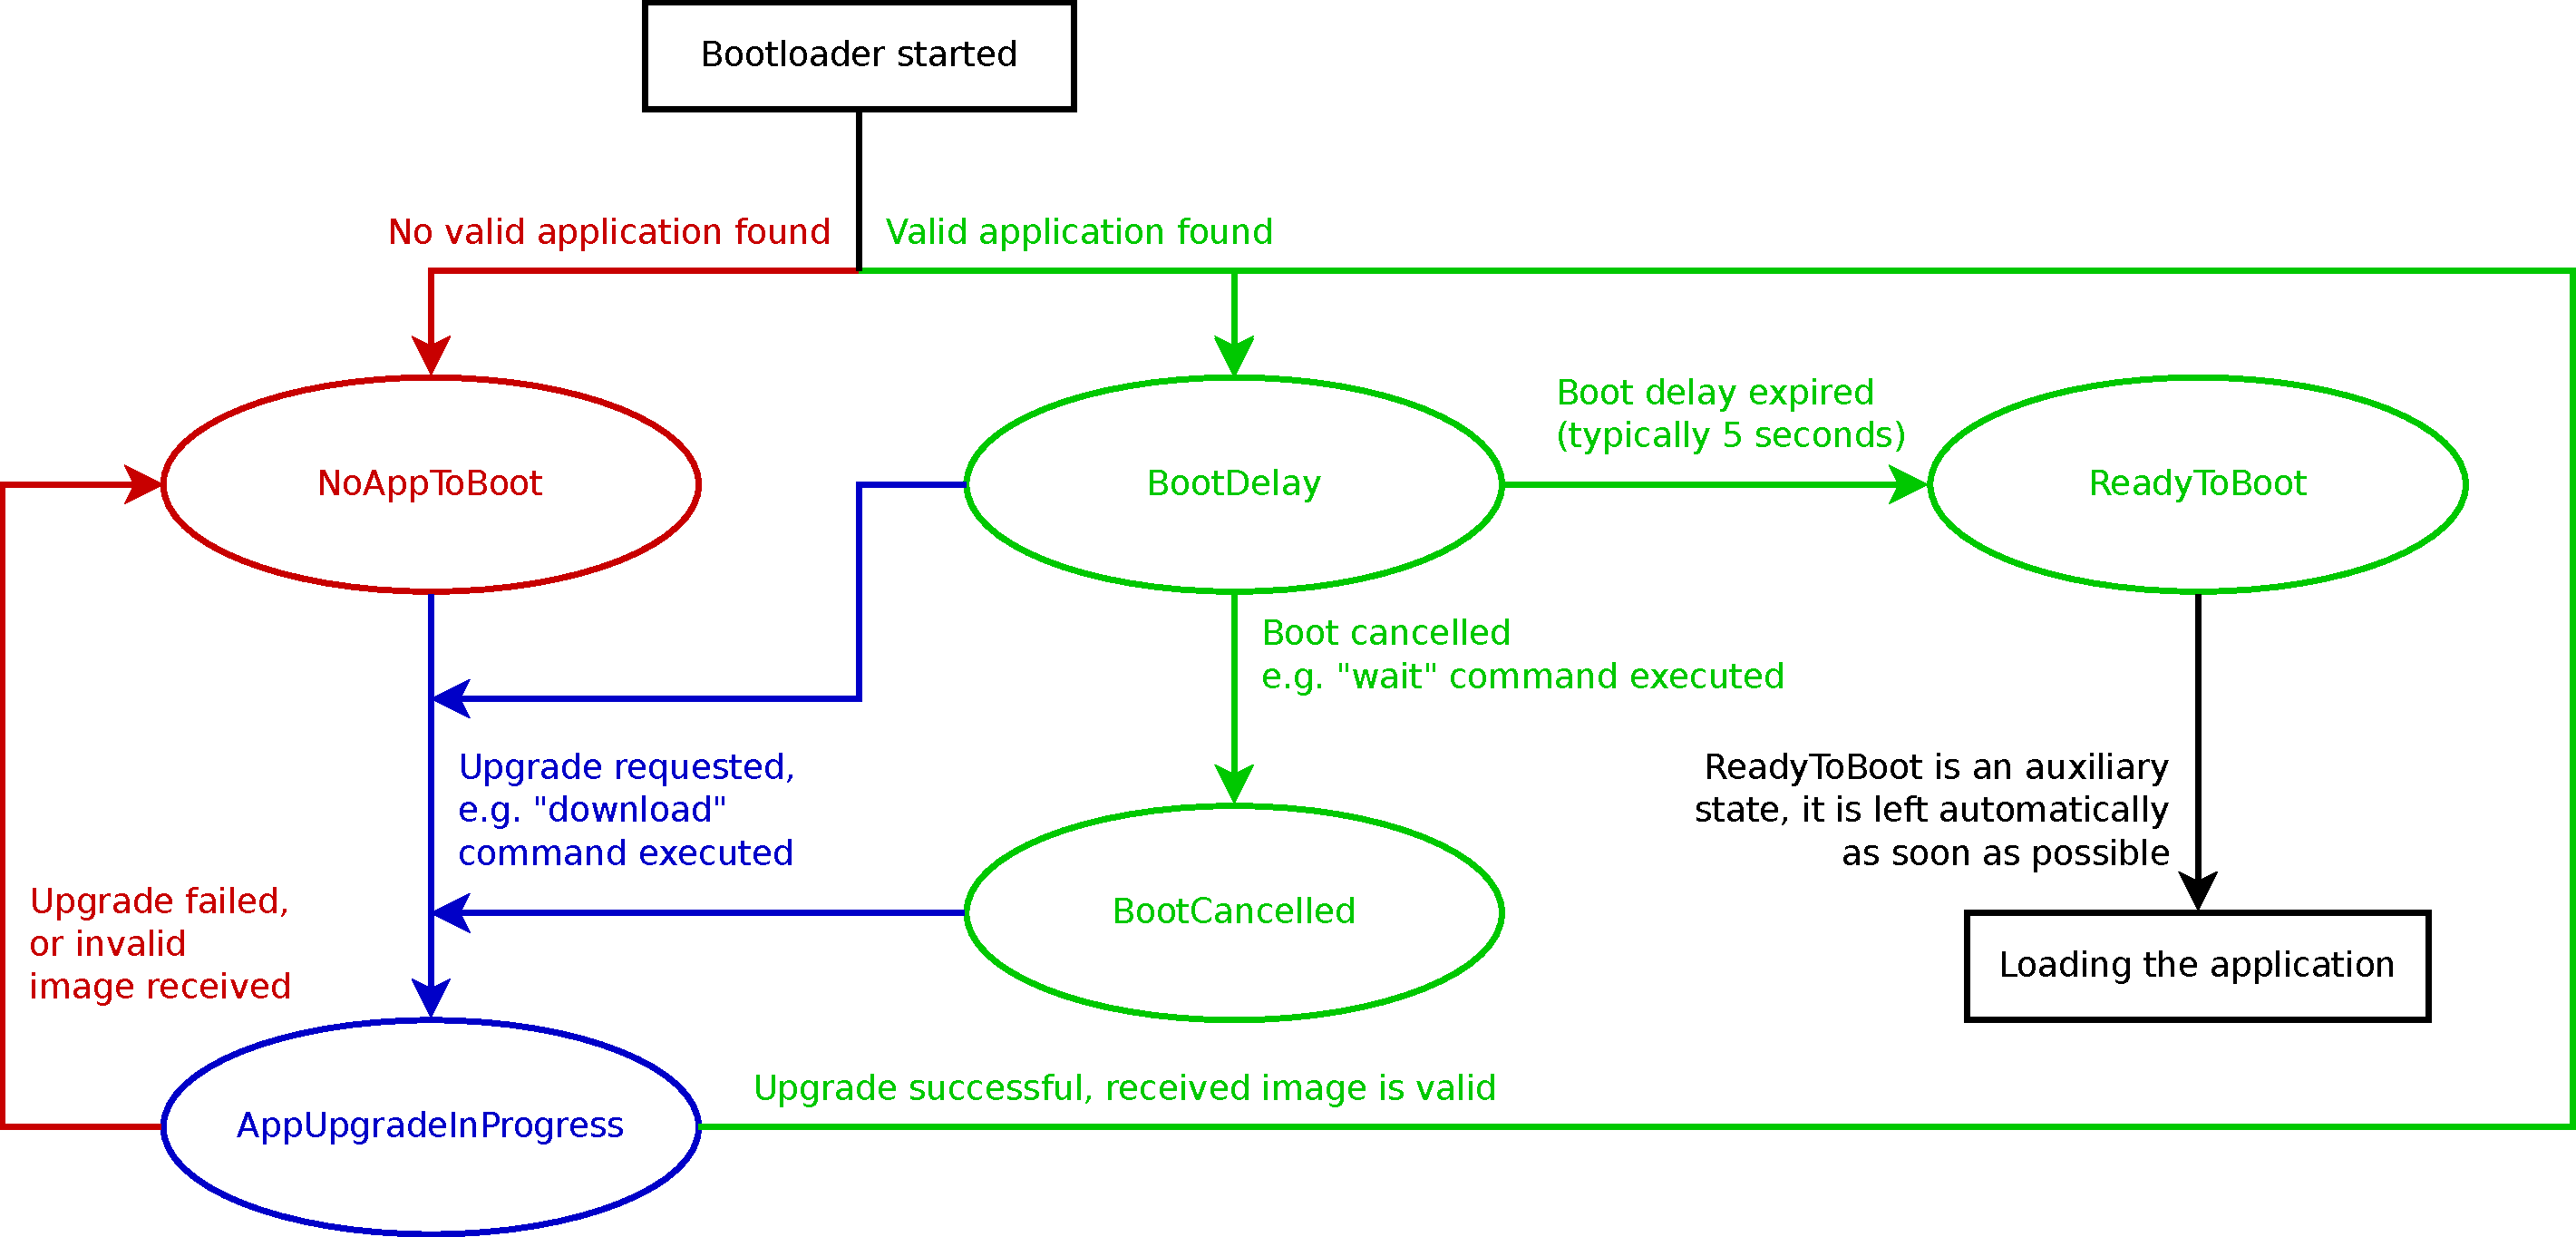
\includegraphics[width=1\textwidth]{bootloader_state_machine}}
	\caption{Bootloader state machine.\label{drawing}}
\end{figure}

\fbox{wait}

Do not boot the application.

\fbox{download}

Start the serial receiver and prepare to receive the new firmware image as a flat binary via the serial link using either YMODEM, XMODEM, or XMODEM-1K. There are heaps of software products and scripts that support these protocols. For instance, the standard program \fbox{sz} can be used as follows:

\begin{minted}[linenos = false]{yaml}
sz -vv --ymodem --1k $file > $port < $port
\end{minted}

If the application was successfully received and CRC verification confirmed that it is not damaged, the bootloader will automatically transition into the state \fbox{BootDelay}.

\iffalse
\chapter{Accessories}

Zubax Babel can be used with the following accesories:
\begin{itemize}
\item \href{https://github.com/Zubax/zubax_babel/tree/master/hardware/enclosure}{Enclosure (suitable for 3D printing)}
\item \href{https://docs.zubax.com/uavcan#UAVCAN_Micro_Patch_Cable}{UAVCAN Micro Patch Cable}
\item \href{https://docs.zubax.com/uavcan#UAVCAN_Micro_to_DF13_Adapter_Cable}{UAVCAN Micro to DF13 Adapter Cable}
\item \href{https://docs.zubax.com/zubax_babel#UAVCAN_Micro_to_D-SUB_DB9F_CAN_Adapter_Cable}{UAVCAN Micro to D-SUB DB9F CAN Adapter Cable}
\end{itemize}

The acessories can be purchased from \href{https://zubax.com/sales-network}{our distributors}.

\chapter{Links}
\begin{itemize}
\item \href{http://shop.titaneliteinc.com/index.php?route=product/product&product_id=1004}{Purchase}
\item \href{https://github.com/Zubax/zubax_babel}{Source repository (includes 3D printable enclosure models)}
\item \href{http://zubax.com/product/zubax-babel}{Product description}
\end{itemize}

\fi

\end{document}
